\subsection{Lap-interrupt Funktion}

Lap-interruptet inkrementerer rundetælleren, som vi bruger til at se om vi er i Preround, Mapping round, den første Run time, eller de resterende.



\subsubsection{Lap-interrupt efter Preround}

Her sker intet andet end at vi går videre til Mapping round.

\subsubsection{Lap-interrupt efter Mapping round}

Her går vi fra mapping round til Main round. Når dette sker sammenligner vi det første og det sidste banestykke. Hvis de begge er et sving, eller de begge er et lige stykke, lægges deres længder sammen før det sidste stykke gemmes. Ellers gemmes det sidste stykke først, hvorefter det første stykke gemmes efter det. På denne måde sikre vi os at bilen ikke løber tør for map, hvis længden driver, samt at den ved om banestykket fortsætter forbi målstregen.
\\
Derefter nulstilles mappet så vi kan læse fra det i den rigtige rækkefølge.

\subsubsection{Lap-interrupt Run time}

I alle resterende Lap-interrupts nulstilles mappet blot.

\afterpage{
\begin{figure}
\centering
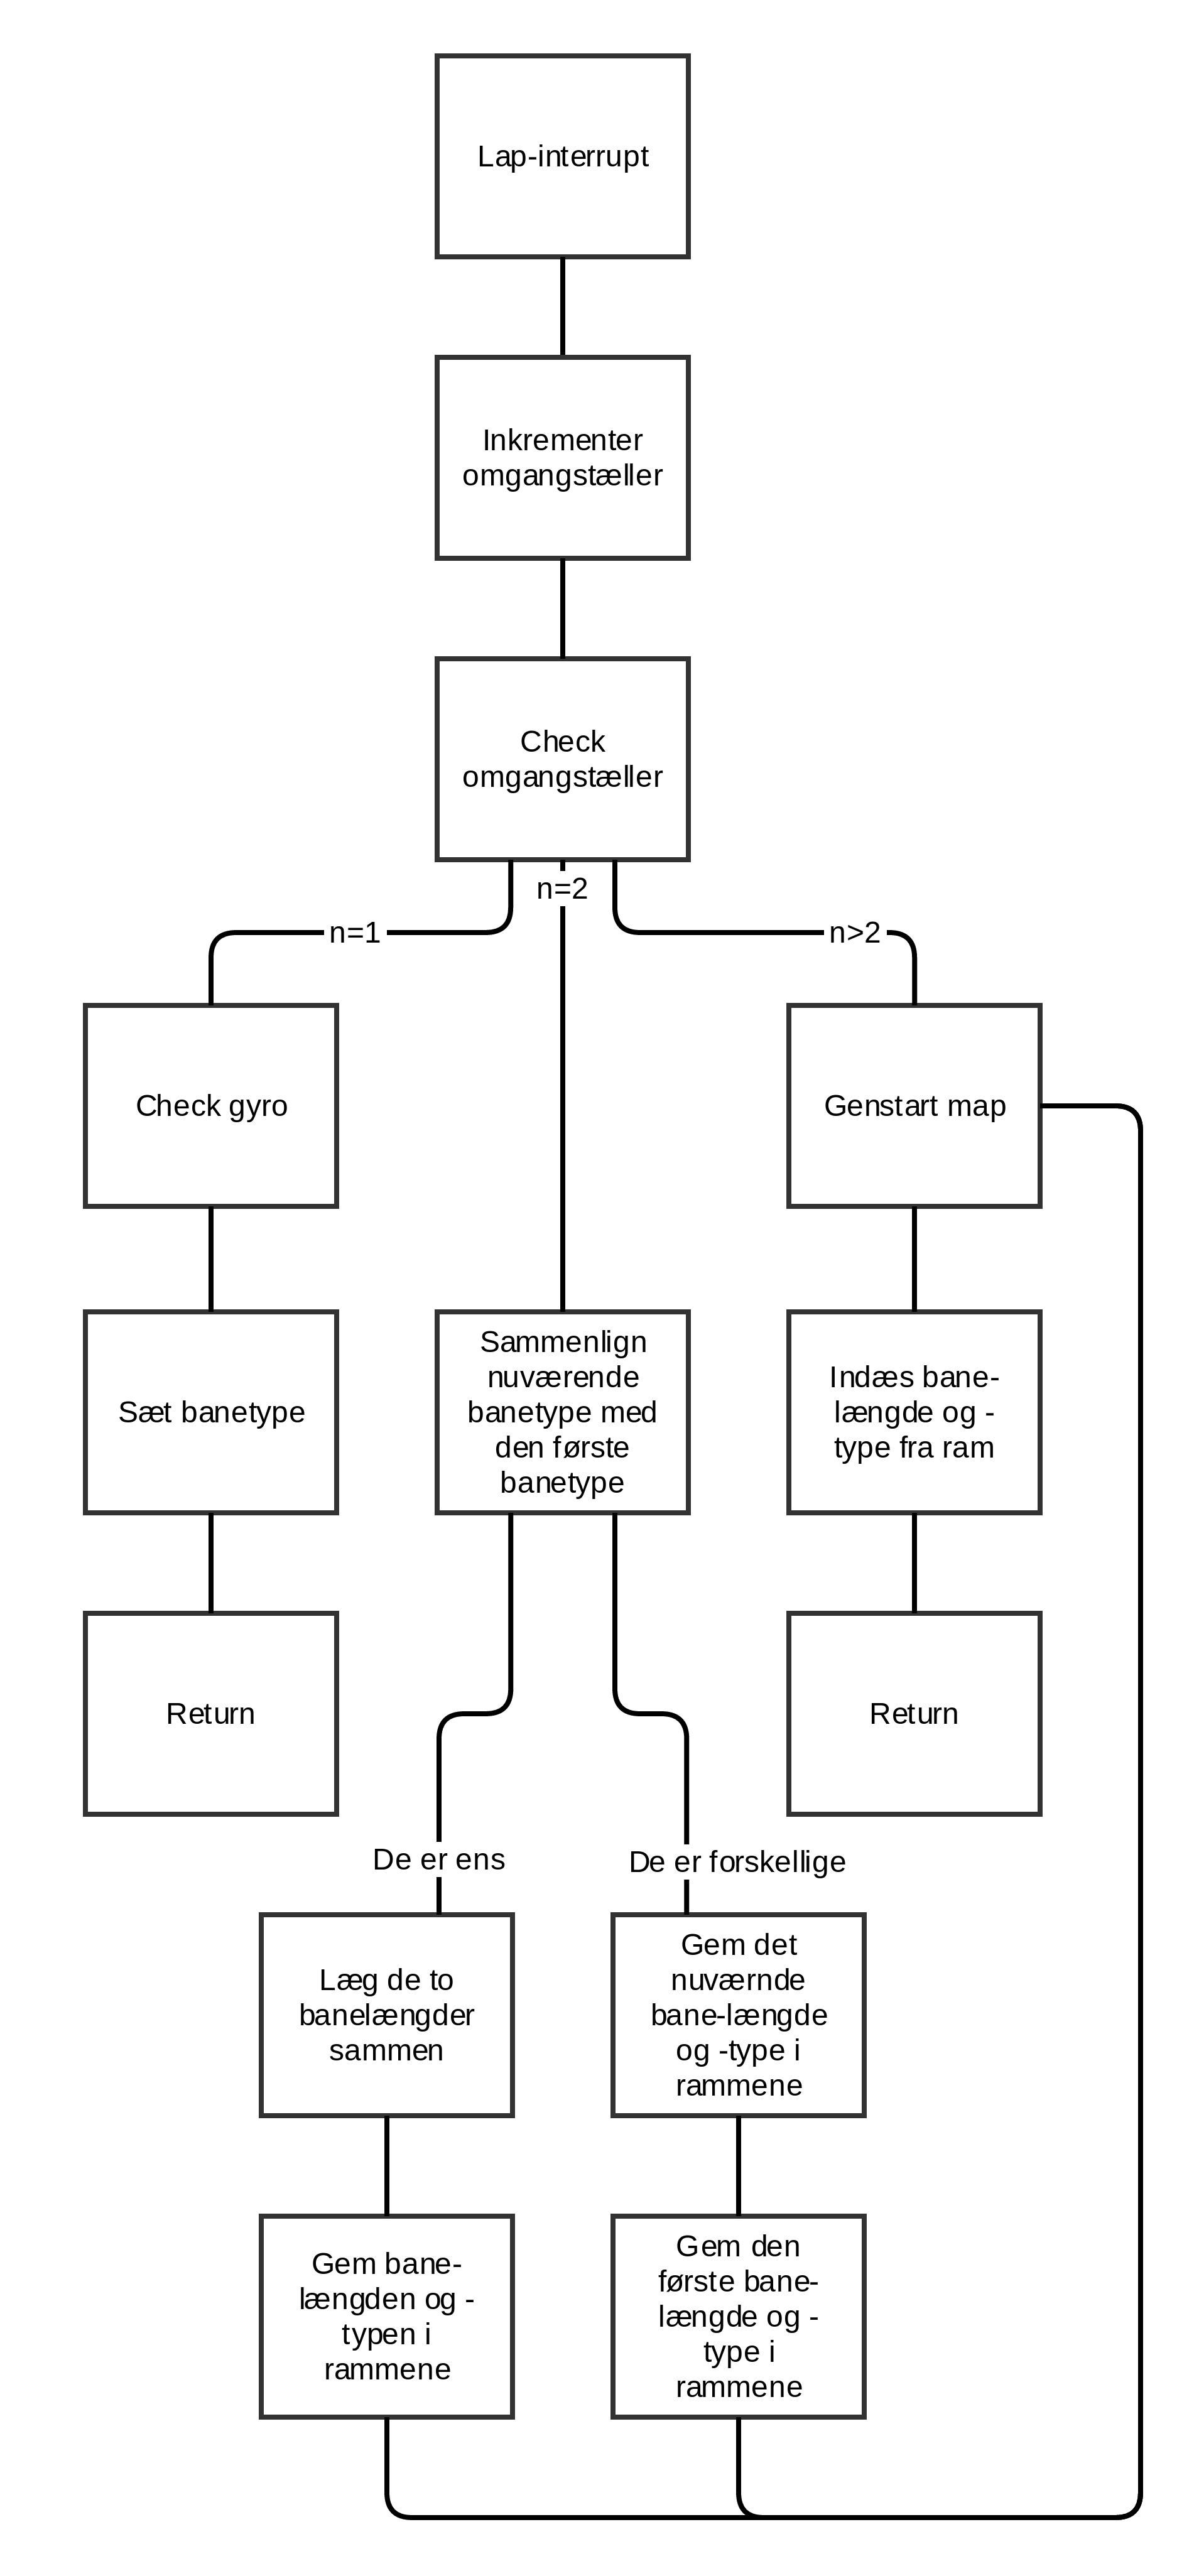
\includegraphics[scale=0.12]{Billeder/lap_interrupt.png}
\caption{Flowchart over Lap-interrupt funktionen.}
\label{fig:Lap Flowchart}
\end{figure}
\clearpage}